\definecolor{genecolor}{RGB}{94,135,173}

\begin{frame}
  \frametitle{Statistical analysis of Networks}
  \framesubtitle{Different questions}

  \begin{block}{Understanding the network topology}
    \vspace{-.25cm}
    \begin{itemize}
    \item Data = observed network
    \item Questions: central nodes? cluster structure? small-world property?
    \end{itemize}
  \end{block}
  
  \vfill

  \begin{alertblock}{Inferring/Reconstructing the network}
    \vspace{-.25cm}
    \begin{itemize}
    \item Data = repeated signal observed at each node
    \item Questions: which nodes are connected?
    \end{itemize}
  \end{alertblock}

  \vfill

  \begin{block}{\alert{Each to be combined with}}
    covariates, time, heterogeneous data set, missing data, ...  
  \end{block}
\end{frame}

\begin{frame}
  \frametitle{Reconstruction and analysis of biological networks} 
  \framesubtitle{E. coli regulatory network}  

  \begin{columns}
    \begin{column}{.4\textwidth}
      \begin{small}
        \begin{block}{Target network}
          Relations between genes and their products
          \begin{itemize}
          \item highly structured
          \item always incomplete
          \end{itemize}
        \end{block}
      \end{small}
      \begin{small}
        \begin{block}{Data and method}
          \begin{itemize}
          \item transcriptomic data
          \item \alert{Inference}: sparse Gaussian graphical model
          \item \alert{Analysis}: Stochastic Block Model
          \end{itemize}
        \end{block}
      \end{small}
    \end{column}
    \begin{column}{.55\textwidth}
      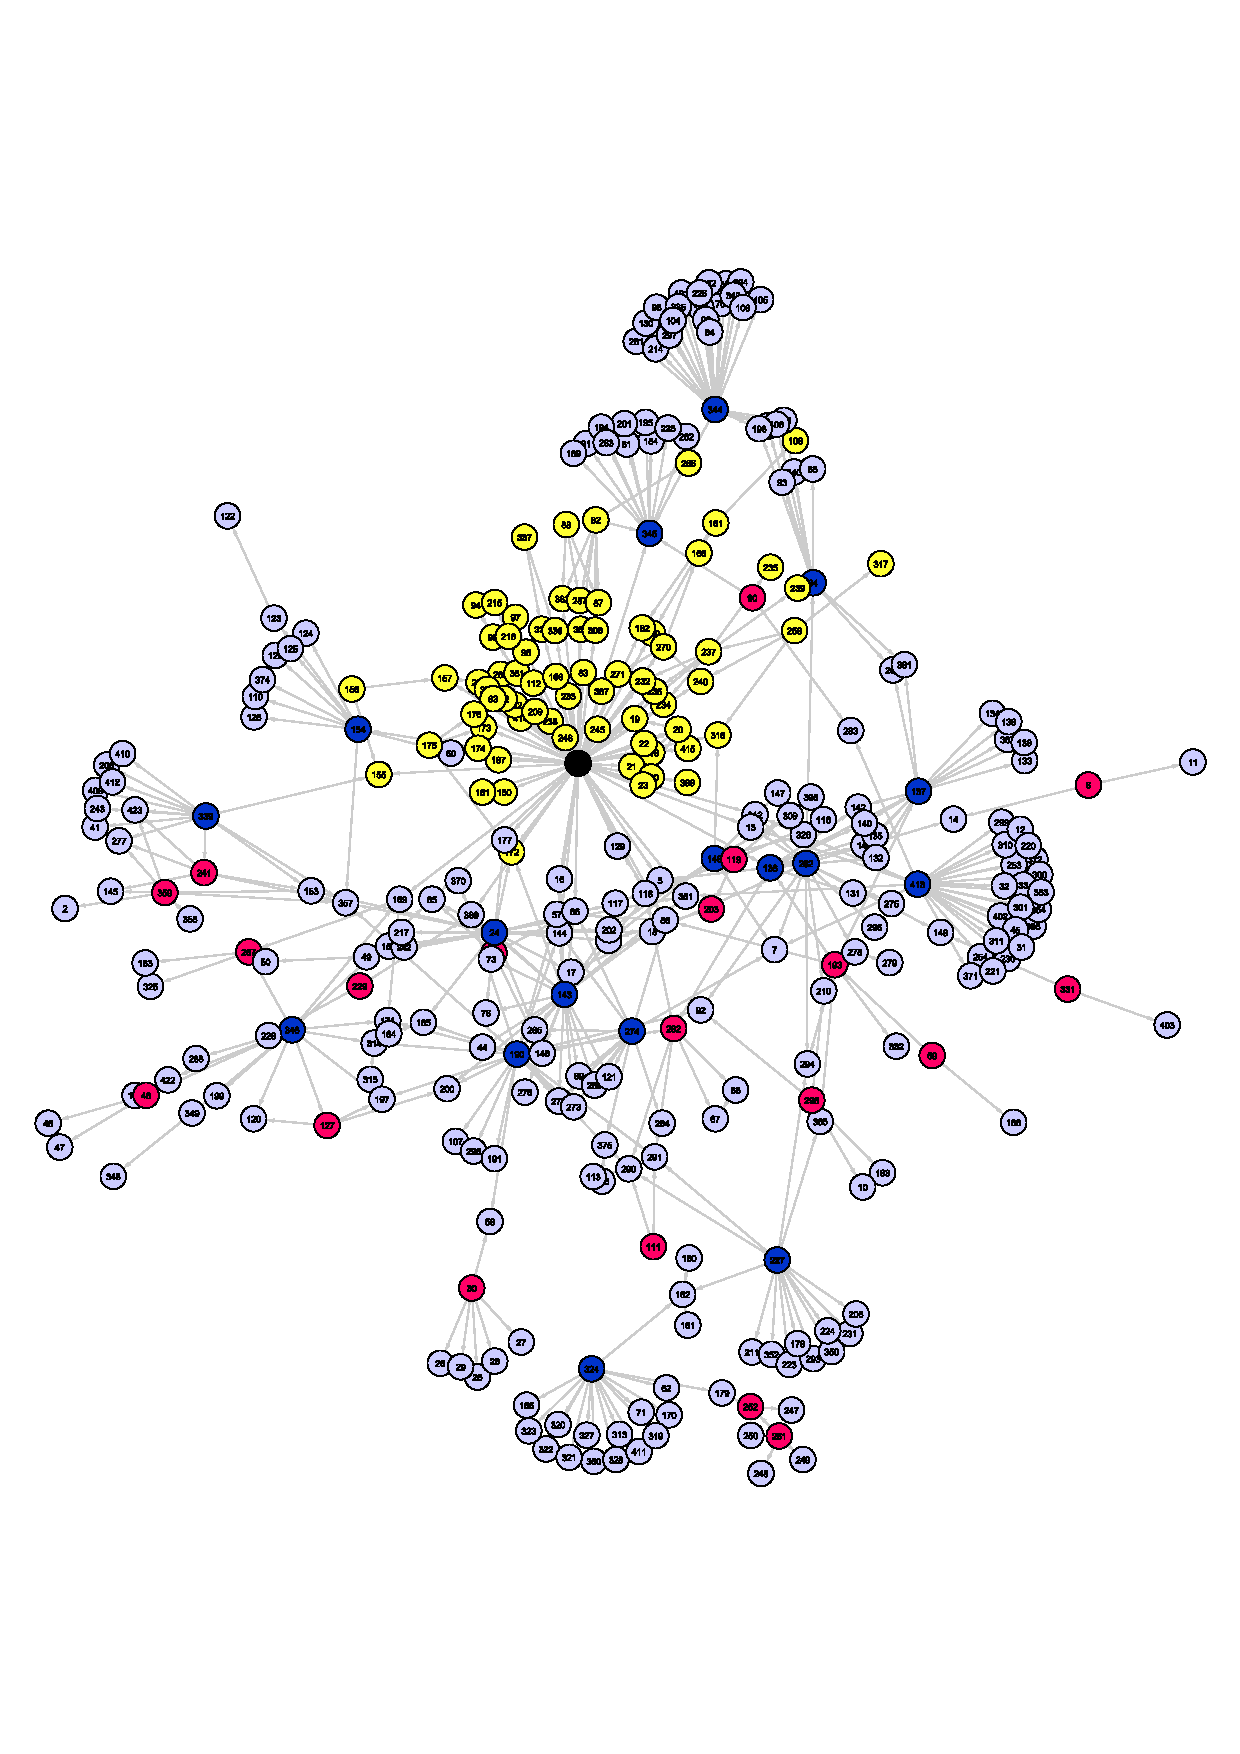
\includegraphics[width=\textwidth]{figures/net_reg_ecoli}
    \end{column}
  \end{columns}
\end{frame}

\begin{frame}
  \frametitle{A challenging problem}

  \vspace{-.25cm}

  \begin{columns}[c]
    \begin{column}{.55\textwidth}
      \begin{tikzpicture}[scale=0.75]
        \node[scale=0.75,opacity=0.75] at (-3,3) {\pgfuseimage{sequencer}};
        \node[scale=0.75] at (-3.5,1) {\pgfuseimage{affymetrix}};
        \node[scale=0.75,fill=red, text=white,single arrow] 
        (inference) at (-1.7,1.7) {\sf \scriptsize Inference}; 
        
        \node at (-3,-0.5) {\begin{tabular}{@{}c@{}}
            \tiny $\approx$ 10s/1,000s assays \\ 
            \tiny $\approx $ 1,000s/1,000,000s features \\
          \end{tabular}
        };
        
        %% UN GRAPH 
        \tikzstyle{every edge}=[-,>=stealth',shorten >=1pt,auto,thin,draw,color=genecolor]
        \tikzstyle{every node}=[fill=genecolor]
        \tikzstyle{every state}=[draw=none,text=white,scale=0.5, transform shape] 
        
        % premier cluster
        \node[state] (A1) at (0,1.75) {g1};
        \node[state] (A2) at (1,0.75) {g2};
        \node[state] (A3) at (0,-.25) {g3};
        \node[state] (A4) at (-1,0.75) {g4};
        \node[state] (A5) at (0,0.75) {g5};
        
        \foreach   \name/\angle/\text   in  {B1/234/g6,   B2/162/g7,
          B3/90/g8, B4/18/g9, B5/-54/g10} {
          \node[state,xshift=4cm,yshift=4cm]     (\name)    at
          (\angle:1cm) {\text}; }
        
        \node[state] (B6) at (2,2) {g11};
        \node[state] (C1) at (3,0.5) {g12};
        \node[state] (C2) at (2.2,0) {g13};
        
        \path 
        (A5) edge [bend left] (A1)
        (A5) edge [bend left] (A2)
        (A5) edge [bend left] (A3)
        (A5) edge [bend left] (A4)
        (B6) edge [bend right] (B1) 
        (B6) edge [bend right] (B2) 
        (B6) edge [bend right] (B3) 
        (B6) edge [bend right] (B4) 
        (B6) edge [bend right] (B5) 
        (C2) edge [bend left] (C1)
        (A5) edge [bend left] (B6)
        (B6) edge [bend right] (C2);
      \end{tikzpicture}
    \end{column}
    \begin{column}{.475\textwidth} 
      \begin{block}{Model point of view}
        \vspace{-.25cm}
        \begin{footnotesize}
            \begin{enumerate}
            \item \alert{Nodes} (genes, OTUS, ...)
              \begin{scriptsize}
                \begin{itemize}
                \item \scriptsize fixed variables
                \end{itemize}
              \end{scriptsize}
            \item \alert{Edges} (biological interactions)
              \begin{scriptsize}
                \begin{itemize}
                \item \scriptsize use (partial) correlations or others
                  fancy statistical concepts
                \end{itemize}
              \end{scriptsize}
            \item \alert{Data} (intensities, counts)
              \begin{scriptsize}
                \begin{itemize}
                \item \scriptsize a tidy $n\times p$ dat matrix
                \end{itemize}
              \end{scriptsize}
            \end{enumerate}
            \vspace{-.25cm}
            $\rightsquigarrow$ \alert{Quantities and goals well defined}
          \end{footnotesize}
          \end{block}
    \end{column}
  \end{columns}

  \vspace{-.25cm}
  \begin{block}{Data point of view: \alert{non classical statistics}}<2->
    \vspace{-.25cm}
    \begin{footnotesize}
    \begin{itemize}
    \item (Ultra) High dimensionality ($n<p$, $n\lll p$)
    \item Heterogeneous data
    \end{itemize}
      \end{footnotesize}    
  \end{block}
  \vspace{-.35cm}
  \begin{block}{Biological point of view: \alert{not well defined goals and questions}}<2>
    \vspace{-.25cm}    
    \begin{footnotesize}
    \begin{itemize}
    \item What interaction? Direct? Indirect? Causal?
    \item Whole network? Subnetwork? Groups of key actors?
    \item structured data, mixed data
    \end{itemize}
      \end{footnotesize}    
  \end{block}

\end{frame}

% \begin{frame}
%   \frametitle{Genomic data}
%   \only<1>{\framesubtitle{Microarray technology: parallel measurement of many biological features}}
%   \only<2>{\framesubtitle{Next Generation Sequencing: parallel measurement of \alert{even} many
%     \alert{more} biological features}}
  
%   Focus    e.g.     on    \textit{transcription},    looking    toward
%   \textcolor{genecolor}{\textit{gene regulatory networks}}

%   \begin{tikzpicture}
%     \begin{small}
%       \tikzstyle{every state}=[fill=orange!70!white,draw=none,text=white]
%       \node[state] (dna) at (0,0) {DNA};
%       \node[state] (rna) at (4,0) {RNA};
%       \node[state] (tf) at (6,-0.25) {TF};
%       \node[draw=none,text=white,fill=genecolor, scale=0.75] (gene) at (0.5,0.5) {genes};
%       \node[draw=none,text=genecolor,fill=white] (alter) at ($(dna.south) -(0,3mm)$) {altered?};

      
        
%       \path
%       (dna) edge [->] node[above] {\alert{transcription}} (rna) 
%       (tf) edge [bend left, ->] node[midway] {\textcolor{genecolor}{regulates}} ($(rna.west) -(5mm,0)$)
%       (rna) edge [-,line width=2pt,draw=white,bend left] ($(rna.west) -(15mm,0)$)
%       (rna) edge [bend left, ->] node {\textcolor{genecolor}{regulates}} ($(rna.west) -(15mm,0)$);
%     \end{small}

%     \begin{pgfonlayer}{background}
%       \filldraw [line width=4mm,join=round,black!10]
%       (rna.north -| rna.west) rectangle (rna.south -| rna.east);
%     \end{pgfonlayer}

%   \end{tikzpicture}    

%   \only<1>{
%     \begin{tikzpicture}
%       \node at (0,-.25) {\pgfuseimage{affymetrix}};
%       \node[fill=mred, text=white,single arrow] 
%       (sig) at (3.5,-.25) {\sf \scriptsize signal processing}; 
%       \node[opacity=.75] (array1) at (7.25,0.25) {\pgfuseimage{microarray}};
%       \node[opacity=.9] (array2) at (7.5,0) {\pgfuseimage{microarray}};
%       \node[opacity=.95] (array3) at (7.75,-0.25) {\pgfuseimage{microarray}};
%       \node at (8,-0.5) (array4) {\pgfuseimage{microarray}};
      
%       \begin{pgfonlayer}{background}
%         \filldraw [line width=4mm,join=round,black!10]
%         (array1.north -| array1.west) rectangle (array4.south -| array4.east);
%       \end{pgfonlayer}
      
%       \node at (7,-3) {%
%         $\mathbf{X} = \begin{pmatrix} 
%           x_1^1 & x_1^2 & x_1^3 & \dots & x_1^p \\
%           \vdots \\
%           x_n^1 & x_n^2 & x_1^2 & \dots & x_n^p \\
%         \end{pmatrix}$};
      
%       \node (output) at (0,-3) { 
%         \begin{tabular}{@{}l@{}}
%           \small Matrix of features $n\ll p$\\ \hline
%           \scriptsize Expression levels of $p$ \\
%           \scriptsize probes are simultaneously \\
%           \scriptsize monitored for $n$ individuals
%         \end{tabular}
%       };
      
%       \begin{pgfonlayer}{background}
%         \filldraw [line width=4mm,join=round,black!10]
%         (output.north -| output.west) rectangle (output.south -| output.east);
%       \end{pgfonlayer}
      
%       \node[fill=mred, text=white,single arrow, shape border rotate =180] 
%       (inference) at (3.35,-3) {\sf \scriptsize pretreatment}; 
%     \end{tikzpicture}    
%   }
  
%   \only<2>{
%     \begin{tikzpicture}
%       \node at (0,-.25) {\pgfuseimage{sequencer}};

%       \node[fill=mred, text=white,single arrow] 
%       (sig) at (3.5,-.25) {\sf \scriptsize assembling}; 
      
%       \node[opacity=.75] (array1) at (7.25,0.25) {\pgfuseimage{ngs}};
%       \node[opacity=.9] (array2) at (7.5,0) {\pgfuseimage{ngs}};

%       \begin{pgfonlayer}{background}
%         \filldraw [line width=4mm,join=round,black!10]
%         (array1.north -| array1.west) rectangle (array2.south -| array2.east);
%       \end{pgfonlayer}
      
%       \node at (7,-2.75) {%
%         $\mathbf{X} = \begin{pmatrix} 
%           k_1^1 & k_1^2 & k_1^3 & \dots & k_1^p \\
%           \vdots \\
%          k_n^1 & k_n^2 & k_1^2 & \dots & k_n^p \\
%         \end{pmatrix}$};
    
%       \node (output) at (0,-2.75) { 
%         \begin{tabular}{@{}l@{}}
%           \small Matrix of features $n\lll p$\\ \hline
%           \scriptsize Expression counts are extracted \\
%           \scriptsize from small repeated sequences \\
%           \scriptsize and monitored for $n$ individuals
%         \end{tabular}
%       };

%       \begin{pgfonlayer}{background}
%         \filldraw [line width=4mm,join=round,black!10]
%         (output.north -| output.west) rectangle (output.south -| output.east);
%       \end{pgfonlayer}

%       \node[fill=mred, text=white,single arrow, shape border rotate =180] 
%       (inference) at (3.35,-2.75) {\sf \scriptsize pretreatment}; 
%     \end{tikzpicture}    
%     }
% \end{frame}

